\documentclass[12pt,a4paper]{article}
\usepackage[utf8]{inputenc}
\usepackage[T1]{fontenc}
%\usepackage[en_uk]{babel}
\usepackage{amsmath}
\usepackage{amsfonts}
\usepackage{amssymb}
\usepackage{graphicx}
\author{rawfiner and Aurélien Pierre}

\title{EIGF: exposure-independent guided filtering}
\begin{document}
\maketitle

\section{Problem to solve}

Notations:\\
$p$: the image to be smoothed (input)\\
$I$: the guide image\\
$q$: the result (output).\\

For each pixel, we compute a and b such as :
\begin{eqnarray}
q_k &=& \bar{a_k}I_k + b_k\\
a_k &=& \frac{cov_k(I,p)}{var_k(I) + \varepsilon}
\\
b_k &=& \bar{p_k} - a_k\bar{I_k}
\end{eqnarray}

When $I = p$, we get:
\begin{eqnarray}
q_k &=& \bar{a_k}p_k + b_k\\
a_k &=& \frac{var_k(p)}{var_k(p) + \varepsilon}
\\
b_k &=& \bar{p_k} - a_k\bar{p_k}
\end{eqnarray}

Let's take a closer look to $a_k$.
$\varepsilon$ aims at controling the amount of smoothing: the higher $\varepsilon$ is, the smoother the result will be.
$\varepsilon$ is involved in the fraction $\frac{var_k(p)}{var_k(p) + \varepsilon}$.
When $var_k(p)$ is very big compared to $\varepsilon$, the ratio is close to 1, there is very little smoothing.
If $var_k(p)$ is very small compared to $\varepsilon$, the ratio is close to 0, there is a lot of smoothing.

If we increase the exposure of $p$ by 1EV to get a new image $s$, we get:
\begin{eqnarray}
s_k &=& 2 \cdot p_k\\
var_k(s) &=& var_k(2 \cdot p) \\
&=& 4 \cdot var_k(p)\\
a_k &=& \frac{var_k(s)}{var_k(s) + \varepsilon}\\
 &=& \frac{4 \cdot var_k(p)}{4 \cdot var_k(p) + \varepsilon}\\
 &=& \frac{var_k(p)}{var_k(p) + \varepsilon / 4}\\
\end{eqnarray}

Adding 1EV, then smoothing with $\varepsilon$, then removing 1EV, is equivalent to running the guided filter with $\varepsilon / 4$.

A border that is in a dark area of the image, and that would be identical \textit{modulo the exposure} to a border in a brighter area of the image, will be smoothed much more by the guided filter.

\section{Towards an exposure-independent guided filter}
To solve this problem, we need $epsilon$ to be exposure-adaptative.

\subsection{rawfiner's first approach}
We propose to define $\varepsilon$ as a function of exposure-dependent quantities: the pixel value, or the value of the local average around the pixel.
These two quantities are accessible without additional performance costs since they must be computed anyway to compute the original guided filter.

We propose the following formula (with $\alpha \in [0,2]$) :
\begin{eqnarray}
a_k &=& \frac{var_k(p)}{var_k(p) + \varepsilon  \cdot  p_k ^ {\alpha}  \cdot  avg_k(p) ^ {2-\alpha}} \label{first-formula}
\end{eqnarray}

Indeed, when $p$ is multiplied by $d$, $p_k$ and $avg_k(p)$ are also multiplied by $d$, and as $var_k(p)$ is multiplied by $d^2$, we need to have this $d^2$ factor in front of $epsilon$.
The value $\alpha$ allows (to be checked in practice) to control the smoothing of fine details.

\subsection{Aurélien's first approach}

We propose to adjust the $\varepsilon$ parameter in order to automatically compensate the variance dependence on the pixel value and the local mean. If we express the exposure of the current pixel as a sub-multiple of a reference pixel, such as $p = d  \cdot  p_{ref}$, we then look for a normalization coefficient $\alpha$\footnote{warning: this is not the same $\alpha$ as in rawfiner's approach} such that:
\begin{eqnarray}
var_k(p) + \varepsilon \alpha &=& var_k(p_{ref}) + \varepsilon \\
var_k(p) + \varepsilon \alpha &=& var_k(p / d) + \varepsilon\\
\varepsilon (\alpha - 1) &=&  var_k(p) \left( \frac{1}{d^2} - 1\right) \\
\alpha &=& \frac{1}{\varepsilon} var_k(p)  \left( \frac{1}{d^2} - 1\right) + 1
\end{eqnarray}

We get:
\begin{eqnarray}
a_k &=& \dfrac{var_k(p)/d^2}{var_k(p) + \alpha \varepsilon}
\end{eqnarray}
with $d = p_k / p_{ref}$. We choose $p_{ref} = 0.18$, for middle grey.

\subsection{Equivalence of the 2 formulas}
Starting from Aurélien's formula, let's replace $\alpha$ by its formula in the $a_k$ expression:
\begin{eqnarray}
a_k &=& \dfrac{var_k(p)/d^2}{var_k(p) + \varepsilon  \cdot  (\frac{1}{\varepsilon} var_k(p)  \left( \frac{1}{d^2} - 1\right) + 1)}\\
&=& \dfrac{var_k(p)/d^2}{var_k(p) + var_k(p)  \left( \frac{1}{d^2} - 1\right) + \varepsilon}\\
&=& \dfrac{var_k(p)/d^2}{var_k(p) + var_k(p)/d^2  - var_k(p) + \varepsilon}\\
&=& \dfrac{var_k(p)/d^2}{var_k(p)/d^2 + \varepsilon}\\
&=& \dfrac{var_k(p)}{var_k(p) + \varepsilon \cdot d^2}
\end{eqnarray}

Let's replace $d$ by its formula:
\begin{eqnarray}
a_k &=&\dfrac{var_k(p)}{var_k(p) + \varepsilon \cdot \frac{p_k^2}{p_{ref}^2}}\\
a_k &=&\dfrac{var_k(p)}{var_k(p) + p_k^2 \cdot \frac{\varepsilon}{p_{ref}^2}}
\end{eqnarray}

As the user choose $\varepsilon$ the way he wants, we can choose
$\varepsilon'=\frac{\varepsilon}{p_{ref}^2}$.
\begin{eqnarray}
a_k &=&\dfrac{var_k(p)}{var_k(p) + \varepsilon'  \cdot  p_k^2}
\end{eqnarray}

Thus, Aurélien's formula is a particular case of rawfiner's formula ($\alpha = 2$). Good to see that we get coherent formula by taking 2 different paths :-)

\subsection{Analysis of $p_k ^ {\alpha}  \cdot  avg_k(p) ^ {2-\alpha}$}
This term of the formula~\ref{first-formula} deserves to be analysed to answer the questions: why having $avg_k(p)$ in the formula, and what is the effect of $\alpha$.

\subsubsection{Analysis 1}
Why using $avg_k(p)$. Let's take the following exemple:

\begin{figure}[h]
\centering
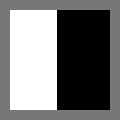
\includegraphics[width=0.1\linewidth]{img/bord}
\caption{Border}
\label{fig:bord}
\end{figure}
Choose 2 pixels in the center of this image, one white pixel and one black pixel.
For these pixels $p_1$ and $p_2$ that are side by side, $var_k(p_1) \approx var_k(p_2)$.
But, using $\alpha = 2$, which means using $p_k^2$ in the formula will five very different smoothing between $p_1$ and $p_2$: the white pixel will be much more smoothed, whereas the neighborhood of the two pixel is identical!
Yet, these 2 pixels have the same local average: using the local average we don't have this issue anymore.
Hence the idea of using $avg_k(p)$.

As a side note, this analysis discourages the use of $p_k$.

\subsubsection{Analysis 2}
Nevertheless, using only $avg_k(p)$ gives a problem in the following case:
\begin{figure}[h]
\centering
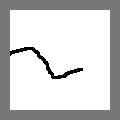
\includegraphics[width=0.1\linewidth]{img/noir_dans_blanc}
\caption{Black detail in a white area}
\label{fig:ndb}
\end{figure}

The black detail in the white area will be strongly smoothed.

\subsubsection{Analysis 3}
In contrast, in the following case, using only $p_k$ gives an oversmoothing:
\begin{figure}[h]
\centering
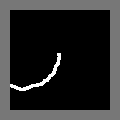
\includegraphics[width=0.1\linewidth]{img/blanc_dans_noir}
\caption{White detail in black area}
\label{fig:bdn}
\end{figure}

The white detail in the black area would be preserved if we used $avg_k(p)$ instead.

\subsubsection{Analysis 4: problem with the use of an average that is not weighted}
\begin{figure}[h]
\centering
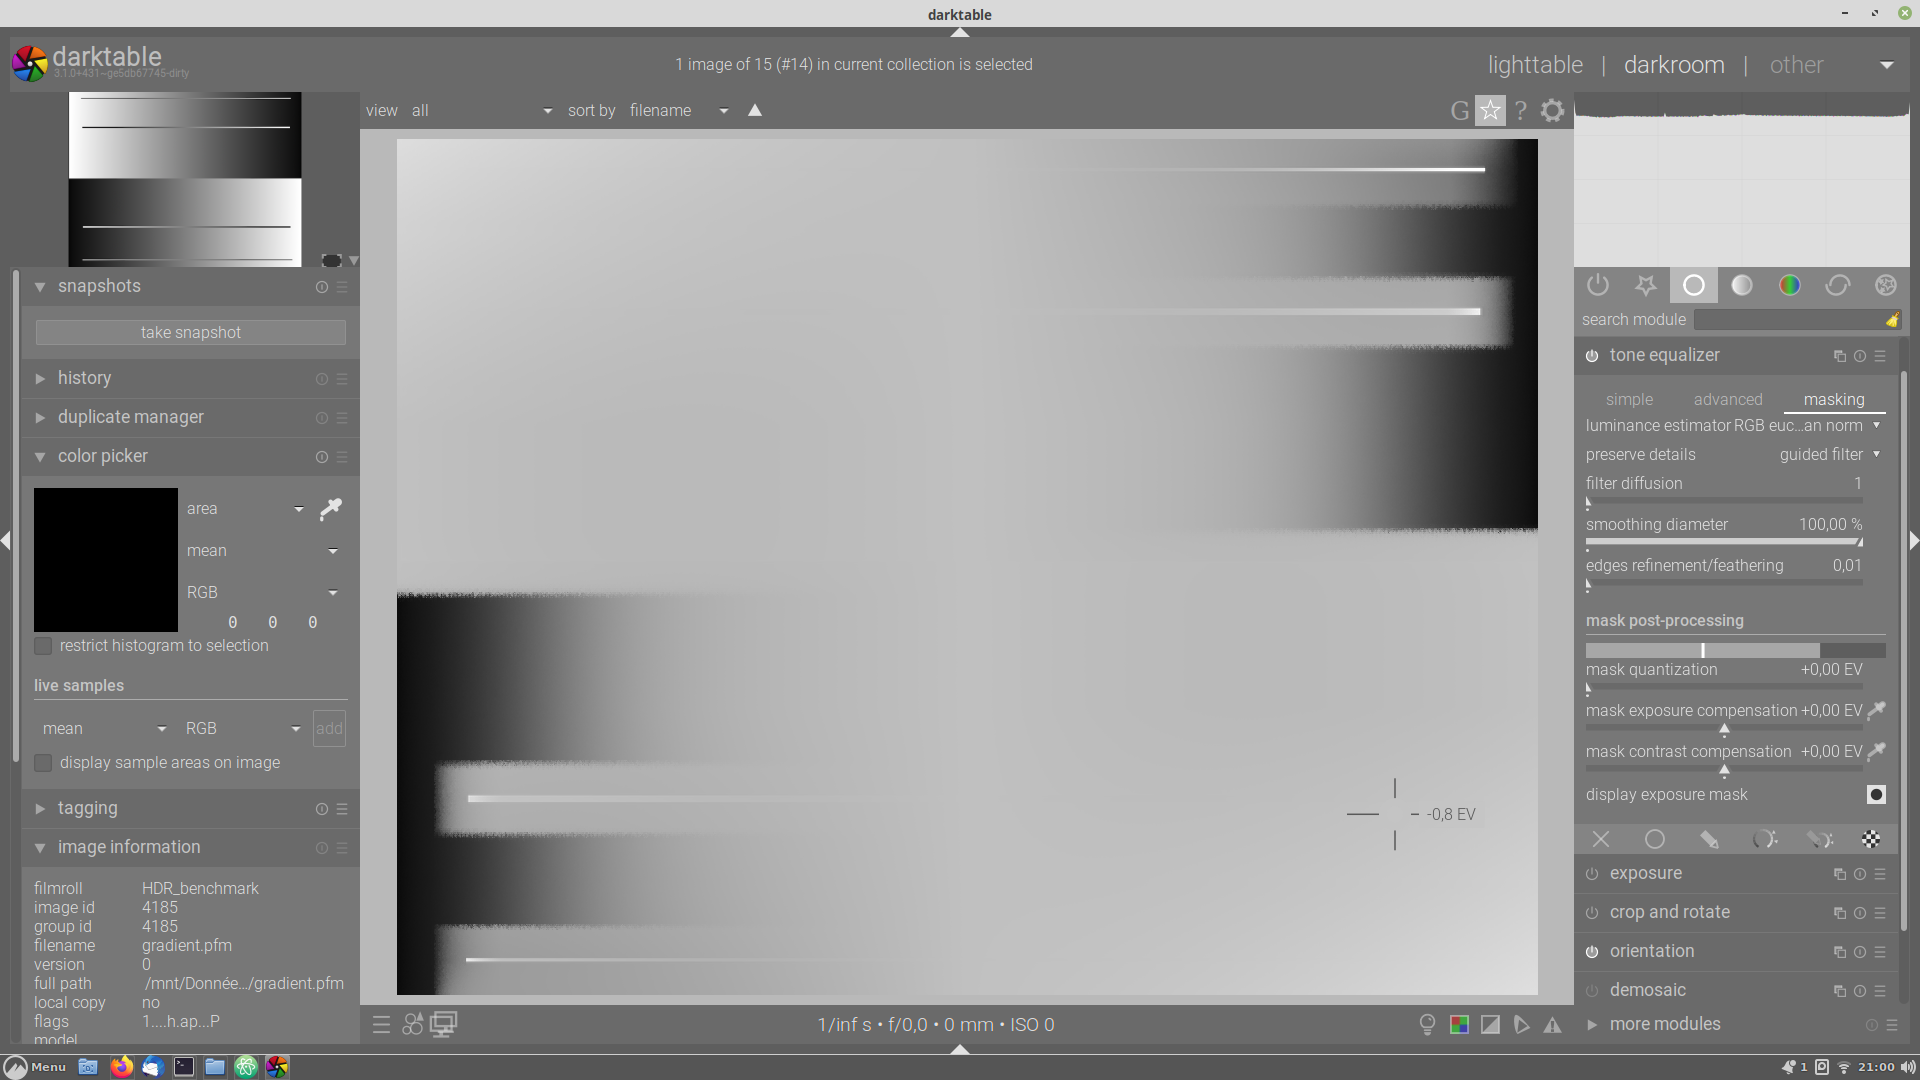
\includegraphics[width=0.7\linewidth]{img/mean1}
\caption{Hard limit parallel to a border}
\label{fig:mean1}
\end{figure}
\begin{figure}[h]
\centering
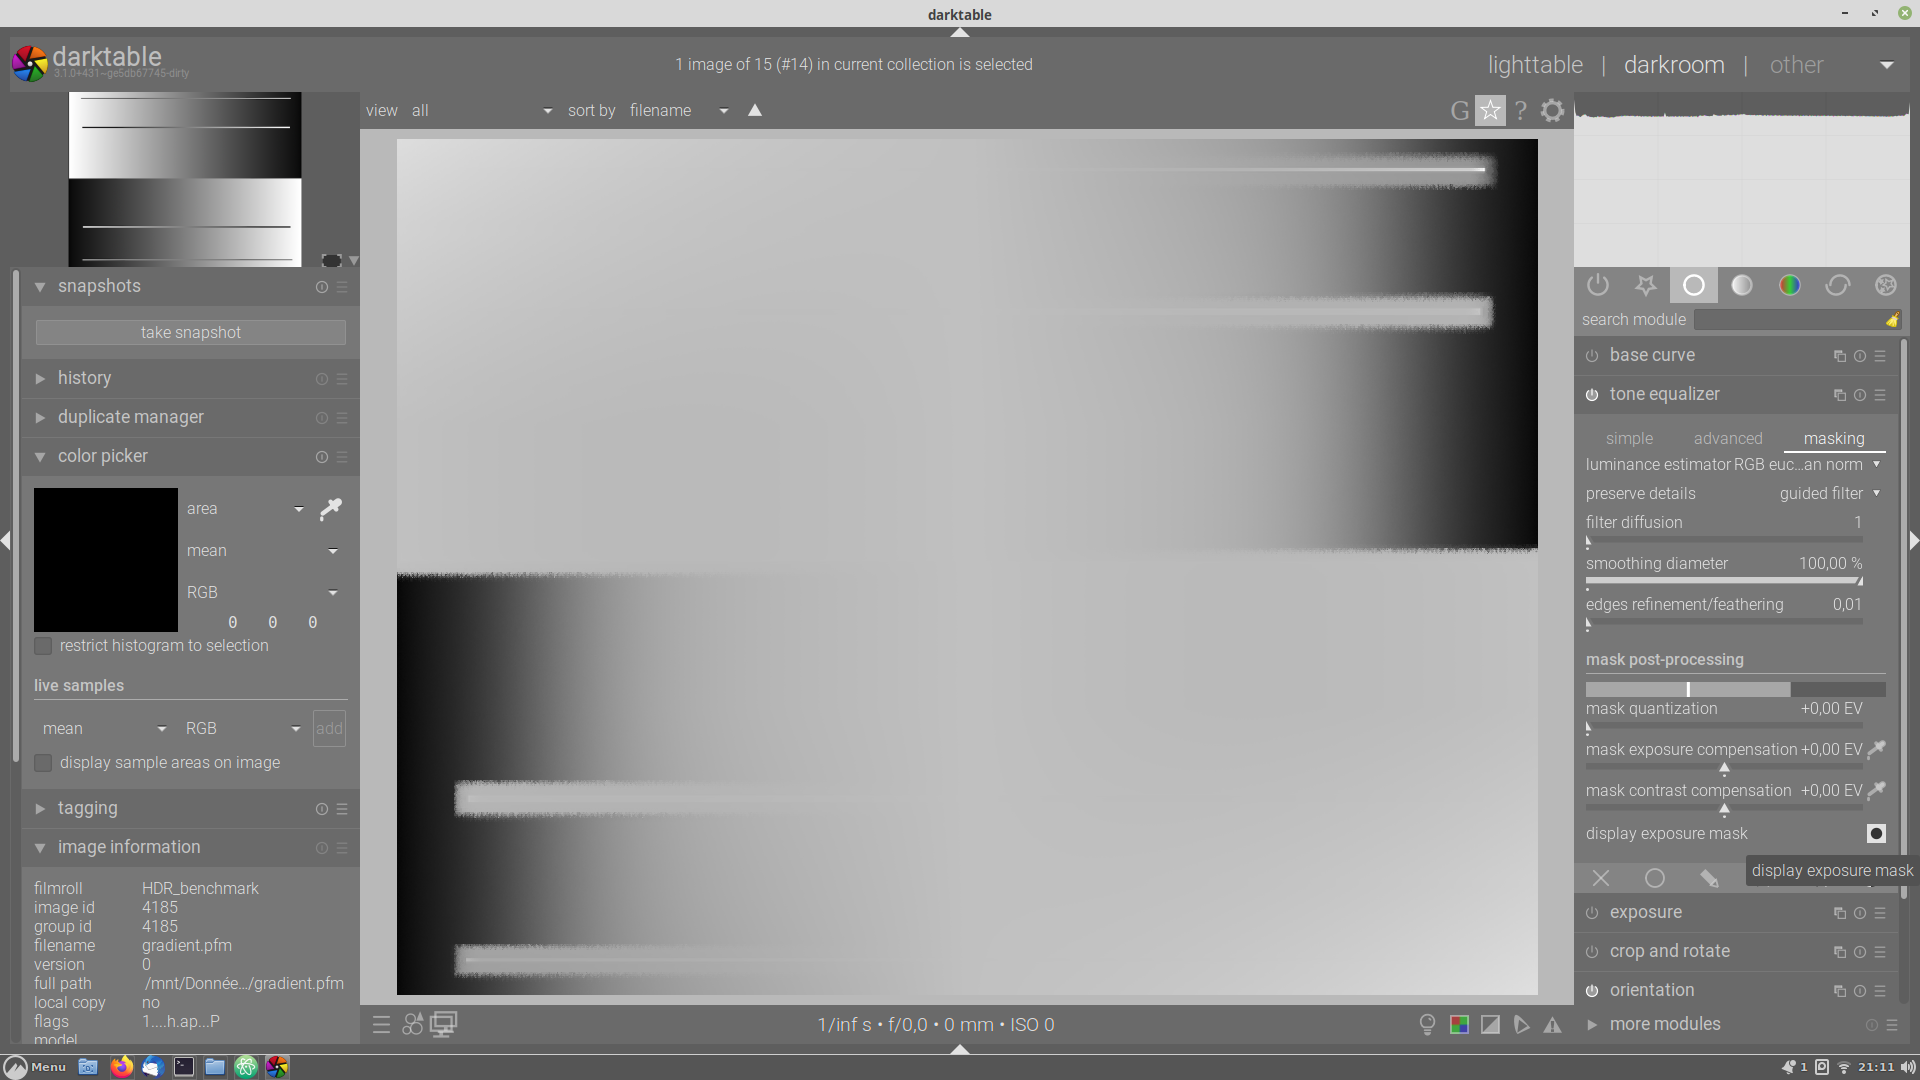
\includegraphics[width=0.7\linewidth]{img/mean2}
\caption{Hard limit parallel to a border, with a mean with a smaller radius}
\label{fig:mean2}
\end{figure}
The use of a local average that is not weighted as exposure-estimator, like the local average used for the guided filter, gives hard limits in zones that do not have any borders, as we can see in figures~\ref{fig:mean1} and~\ref{fig:mean2}.


\subsection{New formula using a gaussian filter to solve all our problems?}
\begin{figure}[h]
\centering
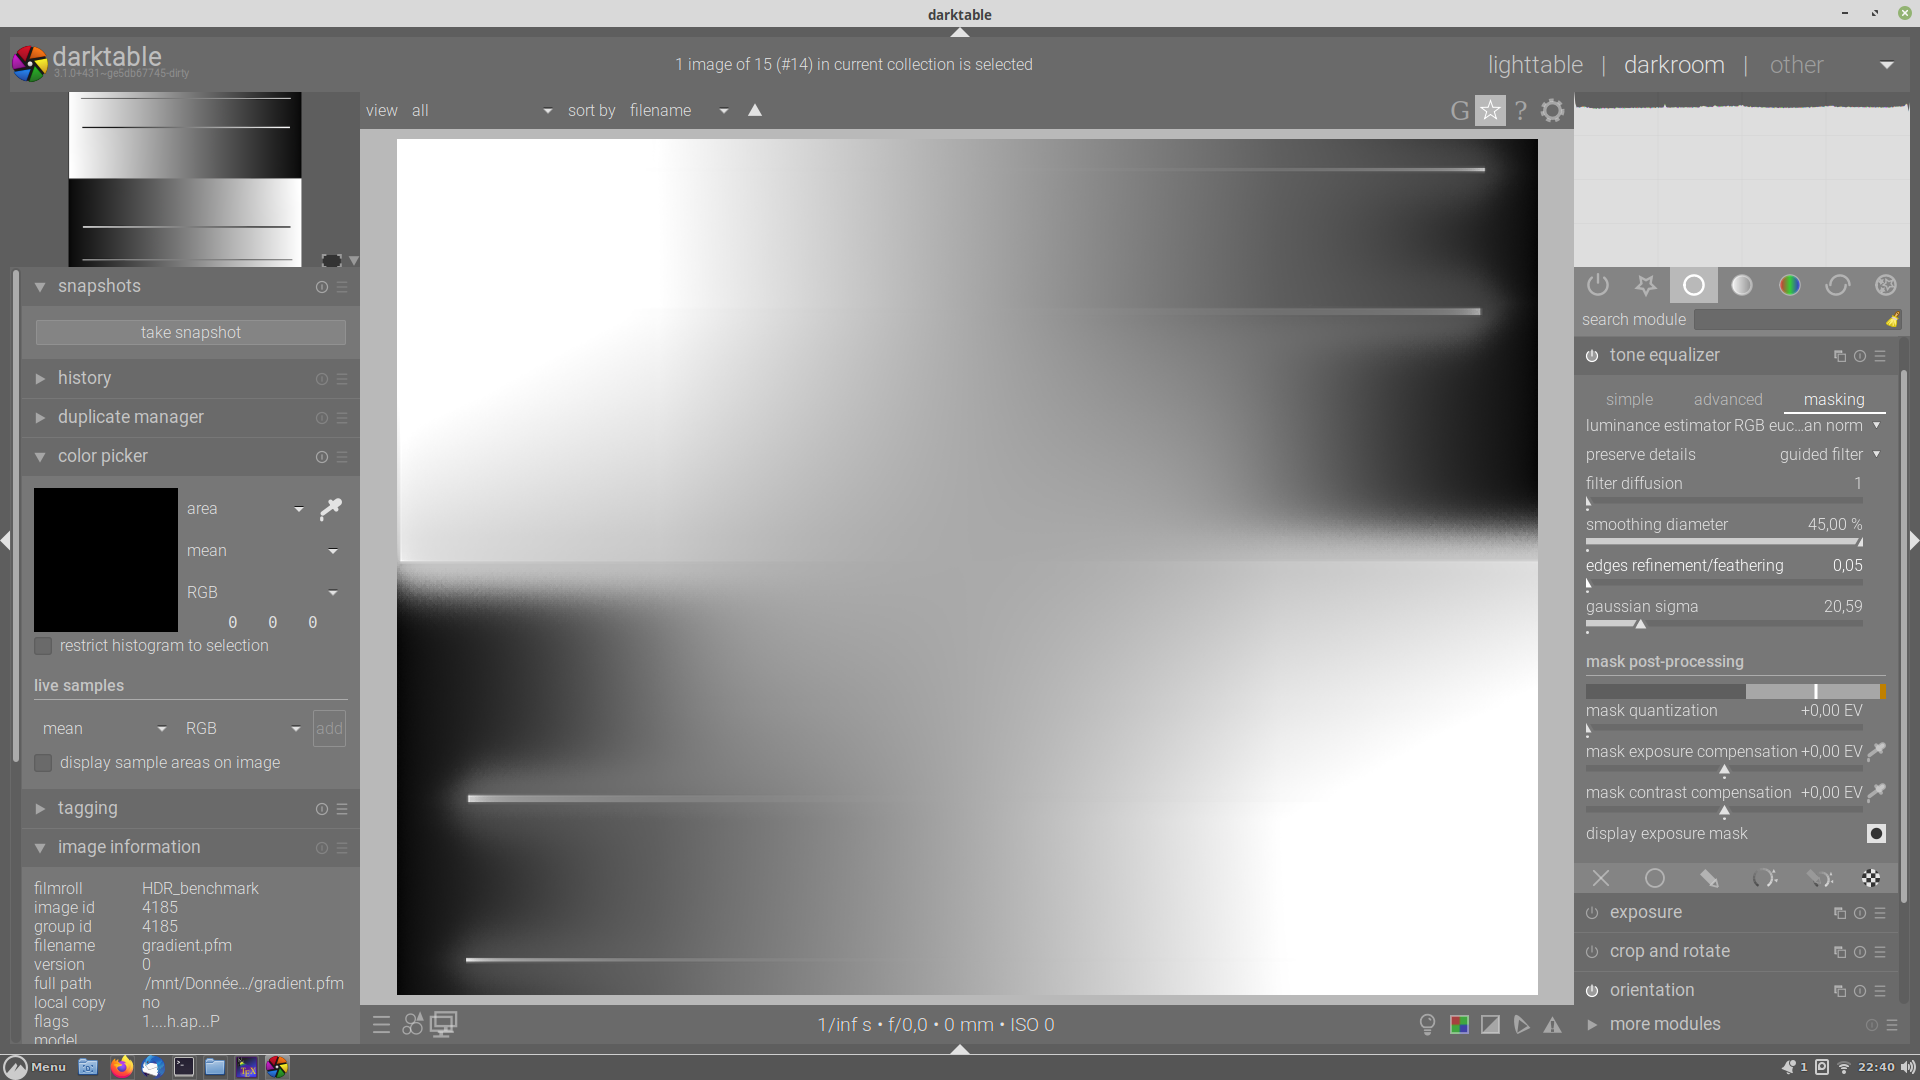
\includegraphics[width=0.7\linewidth]{img/gaussian}
\caption{The result of guided filter do not have hard limits anymore thanks to the use of a gaussian blur}
\label{fig:gaussian}
\end{figure}

To answer our problems, we propose the use of a gaussian blur as a local estimator of the exposure: it allows at the same time to have a continuous average on both sides on a border (analysis 1), and allows to change the weight of central pixel in the blur.
We get a progressif gradient around the edges, as in figure~\ref{fig:gaussian}.

\textbf{We propose the new formula:}
\begin{eqnarray}
a_k &=& \frac{var_k(p)}{var_k(p) + \varepsilon  \cdot  gaussian_k(p) ^ {2}}\label{last-formula}
\end{eqnarray}

The spatial variance of the gaussian blur can be changed by the user to promote the smoothing of shadows or highlights.

\subsection{Box blur of $a_k$}
In the original guided filter, once all $a_k$ are computed, they are averaged using a box blur.

The original paper states: "However, a pixel $i$ is involved in all the overlapping windows that covers $i$, so the value of $q_i$ in (4) is not identical when it is computed in different windows. A simple strategy is to average all the possible values of $q_i$". And later: "The averaging strategy of overlapping windows is popular in image denoising (see [53]) and is a building block of the very successful BM3D algorithm".

In our experiments though, the guided filter behaves much better along the edges if we remove this step, so \textbf{we choose to remove it}.

\subsection{How to test}
\texttt{git clone https://github.com/rawfiner/darktable.git}\\
\texttt{git checkout rawfiner-toneeq}\\

The guided filter within the toneequalizer is updated. In the masking tab, the gaussian sigma slider allows to control the sigma of the gaussian filter of the formula~\ref{last-formula}. It is a log scale. Lowering the value will give better preservation of dark details, while increasing it will give better preservation of bright details.

WARNING: no legacy param conversion has been made! Use with separated database, and test pictures.

\end{document}